\chapter{Energiekalibrierung}
\section{Theoretische Grundlagen}

\subsection{Compton-Streuung}

Die in diesem Versuch eingesetzte $\gamma$-Strahlung stammt aus dem Zerfall von $^{137}$Cs und besitzt eine Energie von etwa $661{,}7\,\mathrm{keV}$. 
In diesem Energiebereich dominiert die Compton-Streuung die Wechselwirkung der Photonen mit Materie. 
Dabei wird ein Photon an einem quasi freien Elektron gestreut und überträgt einen Teil seiner Energie auf dieses Elektron.

Die Energie des gestreuten Photons hängt vom Streuwinkel $\theta$ ab und wird durch die Compton-Beziehung beschrieben \cite{Wermes}:

\begin{align}
    E'_\gamma = \frac{E_\gamma}
    {1+\frac{E_\gamma}{m_e c^2}(1-\cos\theta)}
    \label{eq:compton}
\end{align}

Hierbei bezeichnet $m_e$ die Elektronenmasse und $c$ die Lichtgeschwindigkeit.
\subsection{Photoeffekt}

Der Photoeffekt stellt im Energiebereich der in diesem Versuch verwendeten Gammastrahlung
(einige hundert keV bis etwa 1.5\,MeV) einen der zentralen Wechselwirkungsprozesse zwischen
Photonen und Materie dar. Beim Photoeffekt wird das Gammaquant vollständig von einem
gebundenen Elektron eines Atoms absorbiert. Die gesamte Photonenenergie wird dabei in die
kinetische Energie des Photoelektrons überführt:\cite{Knoll}

\[
E_{\mathrm{kin}} = E_\gamma - E_{\mathrm{Bindung}}.
\]

Das Photoelektron verliert seine Energie anschließend durch Ionisation und Anregung im
Detektormaterial. Im HPGe-Detektor führt dies zur Erzeugung von Elektron--Loch-Paaren,
deren Anzahl direkt proportional zur deponierten Energie ist. Im NaI(Tl)-Detektor erzeugt
das Photoelektron Szintillationslicht, das über den Photomultiplier in elektrische Signale
umgewandelt wird.\\

Da beim Photoeffekt die gesamte Photonenenergie im Detektor deponiert wird, ist er für die
Entstehung der charakteristischen Photopeaks verantwortlich. Diese Photopeaks bilden die
Grundlage der Energiekalibrierung, der Bestimmung der Energieauflösung sowie der
Effizienz- und Aktivitätsanalyse. Ohne den Photoeffekt wäre eine präzise Gammaspektroskopie
nicht möglich, da Compton-Streuung und Paarbildung nur Teilenergien im Detektor
hinterlassen und somit keine scharfen Peaks erzeugen.

Die Wahrscheinlichkeit des Photoeffekts hängt stark von der Ordnungszahl $Z$ des
Detektormaterials sowie der Photonenenergie ab. Näherungsweise gilt:

\[
\sigma_{\mathrm{photo}} \propto Z^n E_\gamma^{-3},
\]

wobei $n$ im Bereich von $4$ bis $5$ liegt. Daraus folgt, dass Materialien mit hoher
Ordnungszahl eine deutlich höhere Photoeffizienz besitzen. Der HPGe-Detektor weist aufgrund seiner geringen Bandlücke und der präzisen Ladungssammlung eine exzellente Energieauflösung auf, jedoch eine geringere Wahrscheinlichkeit für vollständige Energieabsorption.

\subsection{$\gamma$-Spektrum von $^{137}$Cs}

Der Zerfall von $^{137}$Cs erfolgt überwiegend über den angeregten Zustand des
$^{137}$Ba-Kerns, wodurch eine einzelne charakteristische $\gamma$-Linie bei
$661.7\,\mathrm{keV}$ entsteht. Diese Linie bildet im Spektrum den dominanten
Photopeak und eignet sich daher besonders gut für die Energiekalibrierung.

Aufgrund der einfachen Zerfallsstruktur treten beim $^{137}$Cs-Spektrum nur
wenige Überlagerungen auf. Dennoch können Compton-Kontinuum, Rückstreuung
sowie Röntgenlinien des Barium-Tochterkerns zu zusätzlichen Strukturen im
Spektrum führen. Um diese Effekte zu minimieren, wird eine Hintergrundmessung
ohne Probe durchgeführt und vom Spektrum subtrahiert. Dadurch lassen sich
Umgebungsstrahlung, elektronische Störungen und Untergrundereignisse
unterdrücken, sodass der Photopeak klar isoliert werden kann.\cite{Siegbahn}\cite{Knoll}
\subsection{$\gamma$-Spektrum von $^{60}$Co}

Der Zerfall von $^{60}$Co führt über zwei aufeinanderfolgende angeregte Zustände
des $^{60}$Ni-Kerns zu zwei charakteristischen und gut getrennten
$\gamma$-Linien bei $1173\,\mathrm{keV}$ und $1332\,\mathrm{keV}$. Diese beiden
Übergänge besitzen nahezu identische Emissionswahrscheinlichkeiten und bilden
im Spektrum zwei deutlich ausgeprägte Photopeaks.

Aufgrund der höheren Photonenenergien ist das Compton-Kontinuum im
$^{60}$Co-Spektrum besonders ausgeprägt. Die Compton-Kante sowie der
Rückstreupeak sind klar sichtbar und überlagern teilweise den Untergrund im
Bereich zwischen den beiden Photopeaks. Da die Halbwertsbreite des Detektors
mit steigender Energie zunimmt, können sich die Flanken der beiden Peaks
annähern, ohne jedoch zu überlappen.\cite{Siegbahn}\cite{Knoll}


\subsection{$\gamma$-Spektrum von $^{152}$Eu}
Der Zerfall von $^{152}$Eu führt über mehrere angeregte Zustände des $^{152}$Sm zu einer Vielzahl charakteristischer $\gamma$-Linien.\\
Aufgrund der begrenzten Energieauflösung des Detektors können sich mehrere nahe beieinander liegende Übergänge überlappen und einen einzigen Peak bilden. 
Diese Überlappung tritt besonders häufig bei Spannungen über 400 keV auf, da der Linienabstand dann kleiner als die Halbwertsbreite (FWHM) des Detektors ist.
Zur genauen Identifizierung der Linien wird eine Hintergrundmessung ohne Probe durchgeführt und anschließend vom Spektrum subtrahiert, um die Auswirkungen von Umgebungsstrahlung und elektrischem Rauschen zu eliminieren.\cite{Siegbahn}\cite{Knoll}
\begin{table}[H]
\centering
\caption{Literaturwerte der $\gamma$-Energien und relativen Intensitäten von $^{152}$Eu \cite{NuDat3}}
\begin{tabular}{c c}
\hline
$E_{\text{lit}}\,/\,\mathrm{keV}$ & rel.\ Intens.\ $I\,/\,\%$ \\
\hline
121.7817(3)  & 28.53(16) \\
244.6974(8)  & 7.550(40) \\
344.2785(12) & 26.59(20) \\
411.1165(12) & 2.237(13) \\
443.9606(16) & 2.827(14) \\
778.9045(24) & 12.930(80) \\
867.3800(30) & 4.230(30) \\
964.0570(50) & 14.510(70) \\
1085.837(10) & 10.110(50) \\
1112.0760(30) & 13.670(80) \\
1408.0130(30) & 20.870(90) \\
\hline
\end{tabular}
\label{tab_eff_1}
\end{table}



\section{Durchführung}
Im nächsten Schritt werden Gammaspektren der verwendeten radioaktiven Quellen aufgenommen. Konkret werden nacheinander die Spektren von $^{60}Co$, $^{137}Cs$ und $^{152}Eu$ aufgezeichnet. Zusätzlich wird das Untergrundspektrum (ohne Quelle) gemessen, um eine spätere Subtraktion der Untergrundbeiträge zu ermöglichen. Die Messzeiten werden so gewählt, dass die Photopeaks scharf ausgeprägt und statistisch gut aufgelöst sind.\\

Auf der Grundlage der aufgenommenen Spektren wird eine Energiekalibrierung des Systems durchgeführt. Dabei werden die bekannten Gammaenergien der Quellen mit den Kanalnummern verknüpft, die den Photopeaks entsprechen. Mittels linearer Regression wird eine Kalibriergerade bestimmt, die die Umrechnung von Kanalnummern in Energiewerte ermöglicht.

\section{Auswertung}
Die aufgezeichneten Untergrundspektren zeigen eine niedrige Ereignisrate und dominierenden Rauschanteil und wurden von allen Messungen subtrahiert. (siehe Anhang, Abbildung \ref{fig:anhang_1})
Das Untergrundspektrum wurde für jeden Kanal von allen Messungen subtrahiert. Der Untergrundabzug ist notwendig, um Rückstreuanteile und natürliche Radioaktivität zu entfernen, wodurch sonst die Peakflächen systematisch vergrößert werden würden.
Die Peakparameter der verwendeten Kalibrationslinien sind in den Tabellen \ref{HPGe_Caesium}%\ref{HPGe_Cobalt},\ref{NaI_Caesium} \ref{taba_3},
-\ref{NaI_Cobalt} im Anhang zusammengefasst. Diese Werte wurden aus den Fits mit Gaußfunktion und linearem Untergrund gewonnen und bilden die Grundlage für die Energiekalibrierung.

Zur Energiekalibrierung werden Gauß-Funktionen in Kombination mit einem linearen Untergrund an einen begrenzten Kanalbereich um die entsprechenden Photopeaks angepasst. Die verwendete Anpassungsfunktion lautet:
\begin{align}
    G(k) = \frac{A}{\sqrt{2\pi}\sigma}\cdot exp(\frac{-(\mu-k)^2}{2\sigma^2})+a\cdot k +b,\text{ wobei }\sigma_{FWHM}=2\sqrt{2ln(2)}\cdot\sigma
\end{align}
\label{eq_1}

Hier bezeichnet  k den Kanalindex des Vielkanalanalysators (MCA) . Die Ergebnisse ermöglichen die Bestimmung der Peak-Mittenposition $\mu$, der Halbwertsbreite  $\sigma_{FWHM}$ sowie der Peak-Fläche $A$. 

Die folgenden Abbildungen zeigen einen direkten Vergleich der Spektren, die mit beiden Detektoren von derselben Probe aufgenommen wurden. %Zur Erleichterung der Auswertung wurden die Spektren bereits energiekalibriert; die Ergebnisse dieser Kalibrierung werden im weiteren Verlauf vorgestellt. 
Alle durch Gleichung \ref{eq_1} definierten Parameter sind in den Tabellen \ref{taba_2} und \ref{taba_3} aufgeführt. Aufgrund der außergewöhnlichen Schärfe der HPGe-Spektrallinien werden diese zudem in den Abbildungen \ref{fig:anhang_1} detailliert dargestellt.

\begin{figure}[H]
    \centering

    \begin{subfigure}[t]{0.48\textwidth}
        \centering
        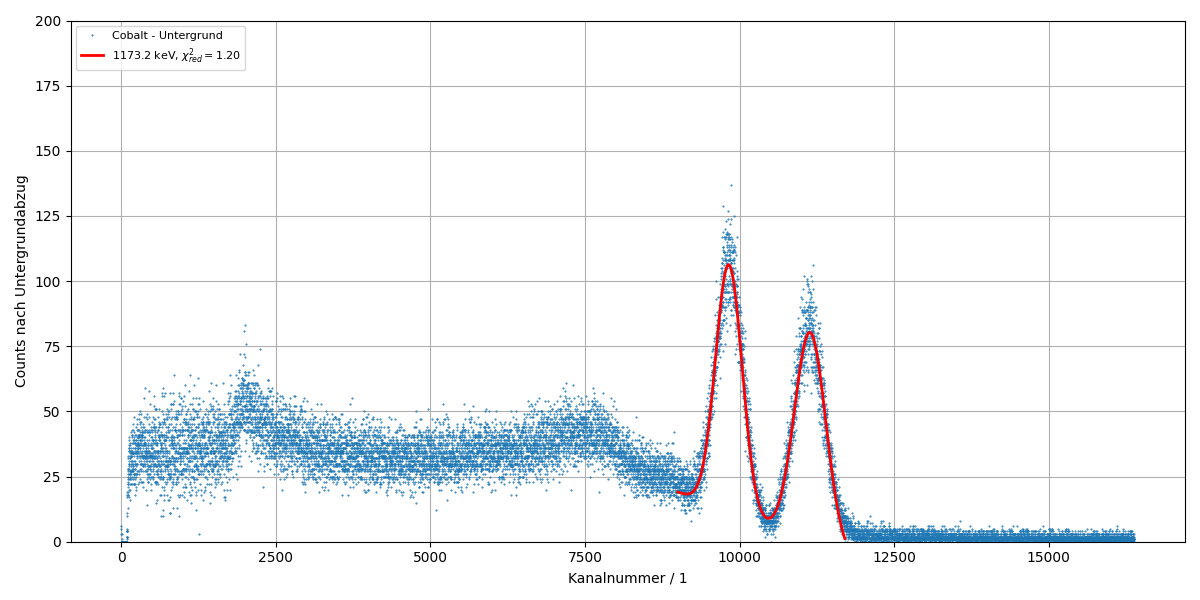
\includegraphics[width=\linewidth]{figs/Cobalt_gausss.png}
        \caption{NaI-Szintillationsdetektor}
        \label{fig:kalib_1_1}
    \end{subfigure}
    \hfill
    \begin{subfigure}[t]{0.48\textwidth}
        \centering
        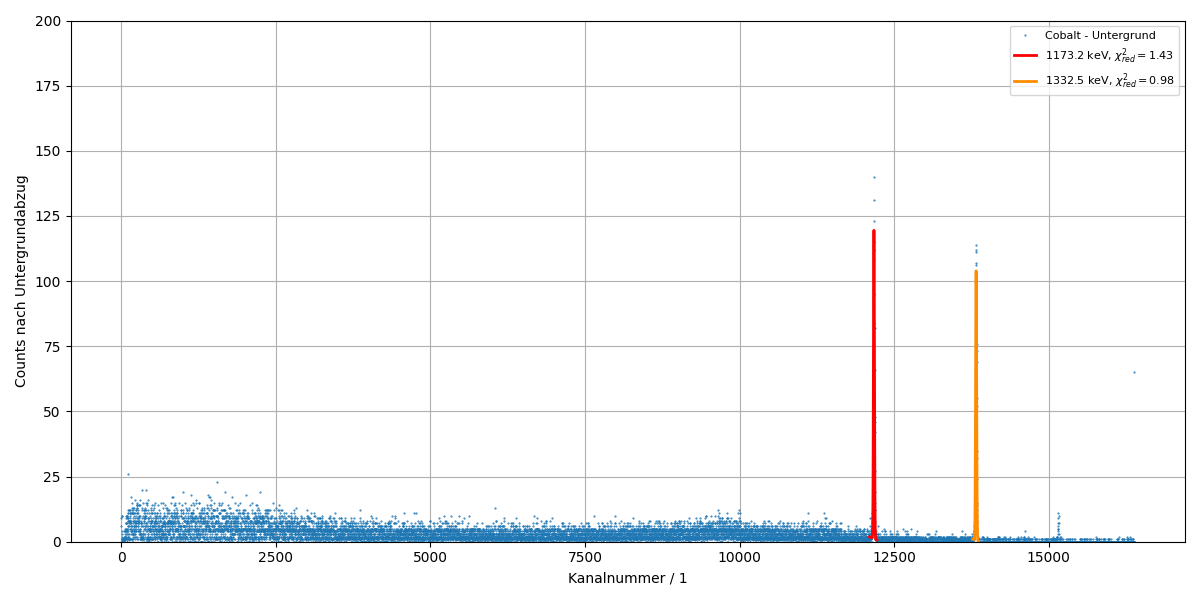
\includegraphics[width=\linewidth]{figs/Ge_Cobalt_gauss.png}
        \caption{HPGe-Halbleiterdetektor}
        \label{fig:kalib_1_2}
    \end{subfigure}

    \caption{Gemessenes Energie-Spektrum der $^{60}$Co-Quelle an beiden Detektoren}
    \label{fig:kalib_1}
\end{figure}
% add plots

% add plots

Auf Abbildung \ref{fig:kalib_1} sind das gemessene Energiespektrum der $^{60}$Co-Quelle an beiden Detektoren zu sehen. Die charakteristischen Linien bei $1173 keV$ und $1332 keV$ sind in den Spektren der HPGe- und NaI-Detektoren deutlich erkennbar.
Es ist ersichtlich, dass der Halbleiterdetektor eine bessere Energieauflösung bietet als der Szintillationsdetektor, was den Erwartungen entspricht. 

Das Compton-Kontinuum resultiert aus dem Compton-Effekt im Detektormaterial: Der Bereich möglicher Streuwinkel $\theta$ (zwischen $0^\circ$ und $180^\circ$) für das gestreute Photon führt zu einer konstanten Verteilung der absorbierten Energie. Die auf das Elektron übertragene Energie erscheint im Spektrum als kontinuierliche Verteilung. Das typische Spektrum weist einen Rückstreupeak bei $(2350\pm100)$ eV, sowie zwei charakteristische Maxima bei $(100\pm50)$ und  $(7500\pm100)$eV, die den extremalen Streuwinkeln $\theta = 180^\circ$ und $\theta = 0^\circ$ entsprechen.\\

Die Cäsium-Spektrum ist in Abbildung \ref{fig:kalib_2} dargestellt. Es zeigt ein ähnliches Verhalten wie die zuvor erwähnten Kobaltspektren und dient der Kalibrierung des 661-keV-Photopeaks.

% add plots
\begin{figure}[H]
    \centering
    \begin{subfigure}[t]{0.48\textwidth}
        \centering
        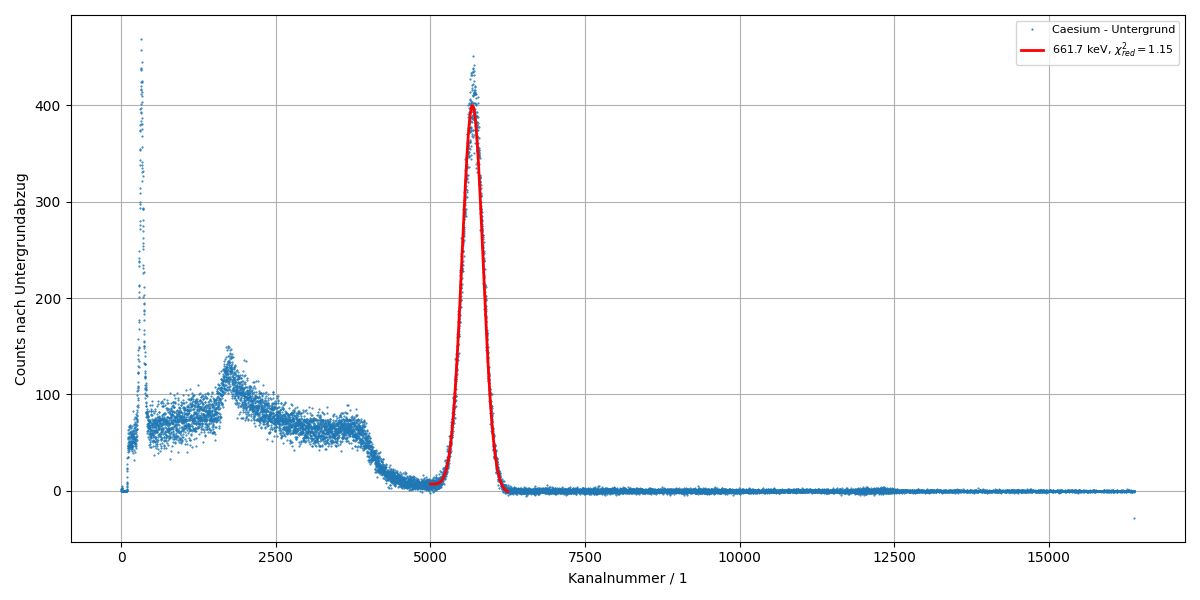
\includegraphics[width=\linewidth]{figs/Caesium_gauss1.png}
        \caption{NaI-Szintillationsdetektor}
        \label{fig:kalib_2_1}
    \end{subfigure}
    \hfill
    \begin{subfigure}[t]{0.48\textwidth}
        \centering
        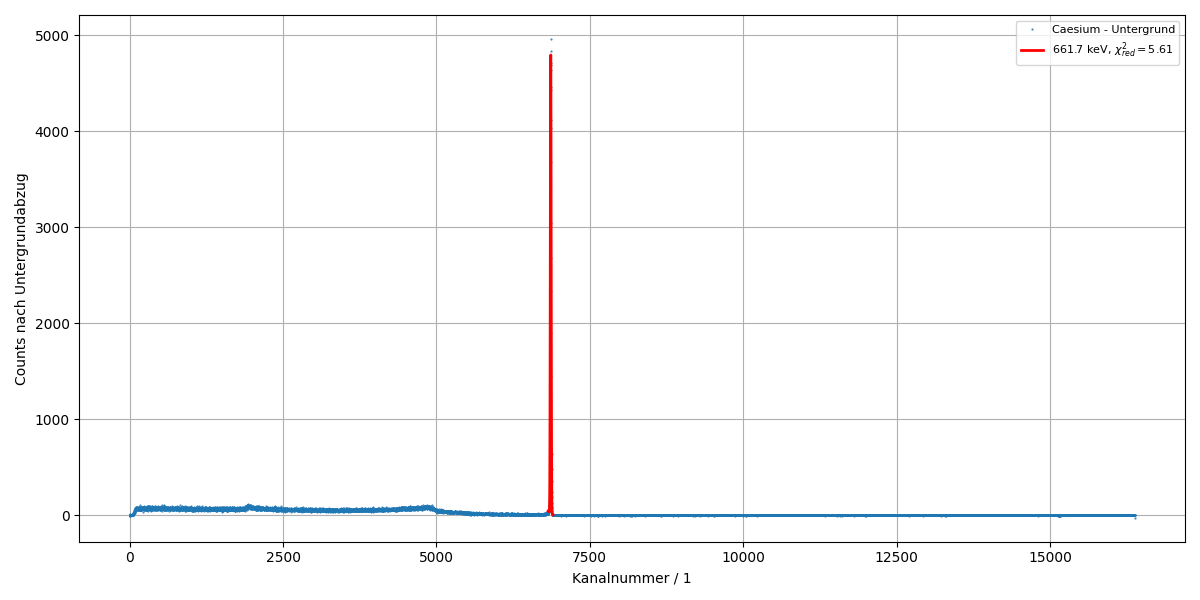
\includegraphics[width=\linewidth]{figs/Ge_caesium_gauss.png}
        \caption{HPGe-Halbleiterdetektor}
        \label{fig:kalib_2_2}
    \end{subfigure}
    \caption{Gemessenes Energie-Spektrum der $^{137}$Cs-Quelle an beiden Detektoren}
    \label{fig:kalib_2}
\end{figure}

Das Europium-Spektrum ist in Abbildung \ref{fig:kalib_3} dargestellt. Es ist deutlich zu sehen, dass beim HPGE-Halbleiterdetektor eine größere Anzahl an Emissionslinien zu beobachten ist. Die Zuordnung der Peaks bezüglich der zu erwartenden Maxima nach Tabelle \ref{taba_2} und \ref{taba_3} ist im Fall des Halbleiter-Detektors gut machbar. Jedoch wird am Szintillations-Detektor jedoch durch die geringe Energie-Auflösung und die geringe Effizienz des Detektors bei hohen Energien erschwert.

\begin{figure}[H]
    \centering
    \begin{subfigure}[t]{0.48\textwidth}
        \centering
        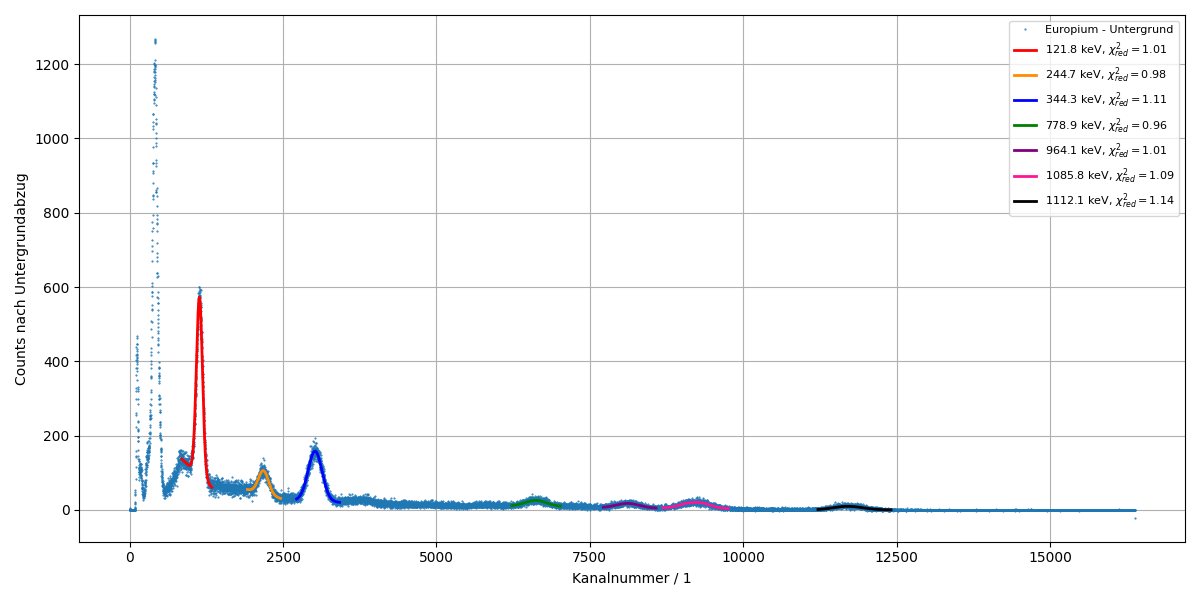
\includegraphics[width=\linewidth]{figs/Europium_gauss3.png}
        \caption{NaI-Szintillationsdetektor}
        \label{fig:kalib_3_1}
    \end{subfigure}
    \hfill
    \begin{subfigure}[t]{0.48\textwidth}
        \centering
        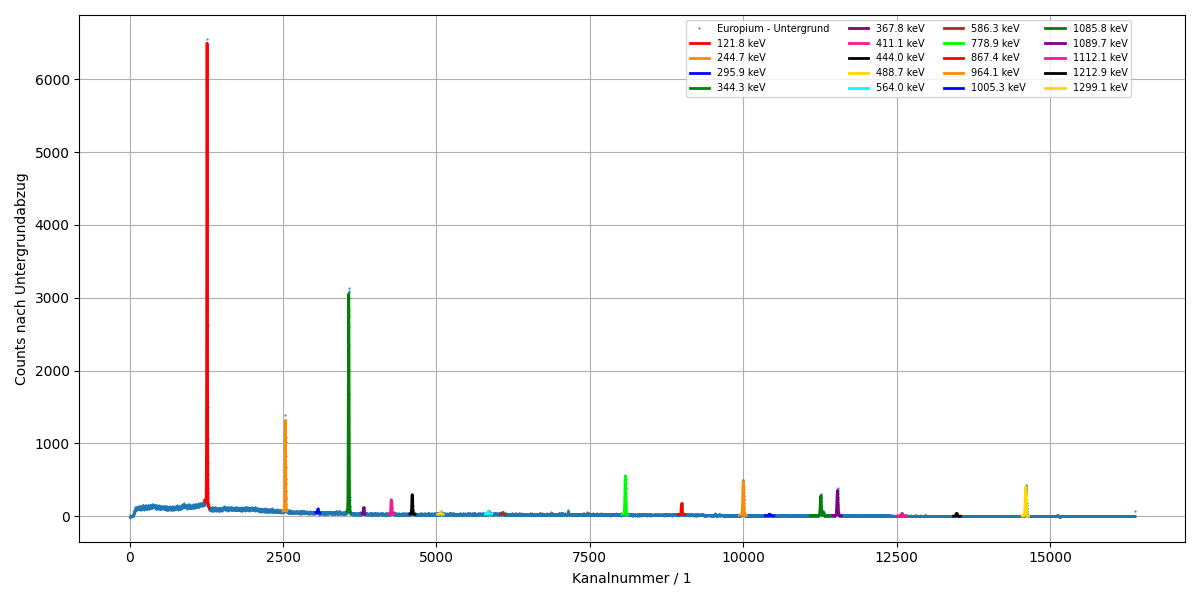
\includegraphics[width=\linewidth]{figs/Ge_Europium_gausss.png}
        \caption{HPGe-Halbleiterdetektor}
        \label{fig:kalib_3_2}
    \end{subfigure}
    \caption{Gemessenes Energie-Spektrum der $^{152}$Eu-Quelle an beiden Detektoren}
    \label{fig:kalib_3}
\end{figure}

% eventuell mehr kommentare

% lineare kalibirierung erklären usw
Es wird eine Energie-Kalibration, unter der Annahme, dass es eine lineare Zuordnung zwischen der Kanalnummer $k$ und der gemessenen Energie $E$ besteht, durchgeführt:
\begin{equation}
    E(k)=\frac{k-b}{a}
\end{equation}
\label{gl:eq_e}
Wenn dies auf die ermittelten Maxima $\mu$ und die Literaturwerte $E(\mu)$ für zugehörigen Energien angewendet wird, ergeben sich
für beide Detektoren die in Abbildung \ref{fig:kalib_4} gezeigten Zusammenhänge:

% add plots
\begin{figure}[H]
    \centering
    \begin{subfigure}[t]{0.48\textwidth}
        \centering
        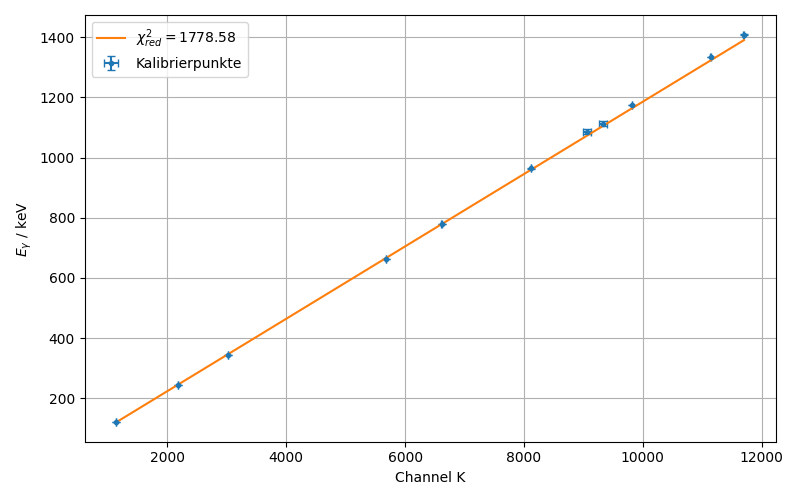
\includegraphics[width=\linewidth]{figs/Energie_kalibrierung.png}
        \caption{NaI-Szintillationsdetektor}
        \label{fig:kalib_4_1}
    \end{subfigure}
    \hfill
    \begin{subfigure}[t]{0.48\textwidth}
        \centering
        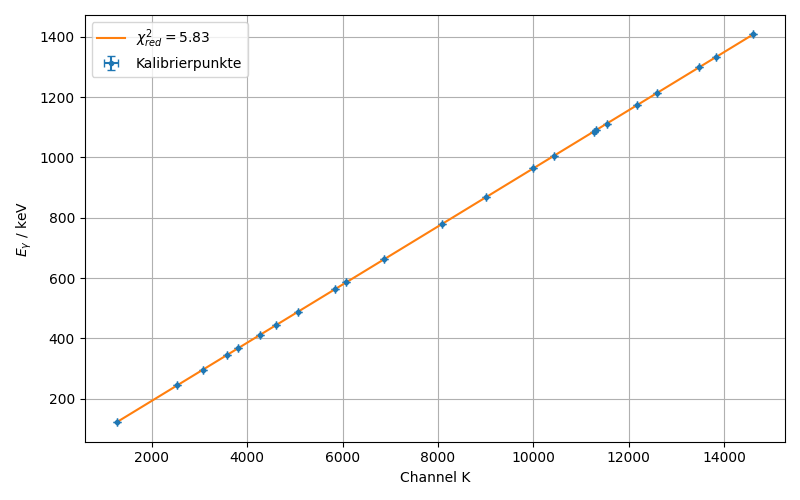
\includegraphics[width=\linewidth]{figs/Ge_Energiekal.png}
        \caption{HPGe-Halbleiterdetektor}
        \label{fig:kalib_4_2}
    \end{subfigure}
    \caption{Energie-Kanal-Kalibration anhand der angepassten $\gamma$-Linien der verwendeten Quellen}
    \label{fig:kalib_4}
\end{figure}
Für den HPGe-Detektor wurden dazu die Linien der $^{137}$Cs, $^{60}$Co und $^{152}$Eu-Quelle verwendet. Beim NaI(Tl)-Detektor wurden aufgrund der geringeren Energieauflösung nur die stärksten, gut getrennten $^{152}$Eu-Linien (121,8; 244,7; 344,3; 964,1 und 1408,0 keV; Tabellen \ref{NaI_Caesium},\ref{NaI_Cobalt}) in die Kalibrierung einbezogen.
Die mit dem linearen Energie-Fit verbundenen Unsicherheiten sind vernachlässigbar, da die Literaturwerte der Übergangsenergien gut bekannt sind und die Positionen der Spektralpeaks mit hinreichender Präzision bestimmt werden können. Die reduzierten Chi-Quadrat-Werte der Peakfits liegen insbesondere beim NaI-Detektor deutlich über dem erwarteten Bereich von $\chi^2_\mathrm{red} \approx 1$. Dies ist wahrscheinlich darauf zurück zu führen, dass die Peaks von Szintillationsdetektoren aufgrund von Lichtsammlungsverlusten und Compton-Anteilen nicht ideal gaußförmig sind. Trotz der großen $\chi^2_\mathrm{red}$-Werte sind die Peakpositionen jedoch robust bestimmt, sodass die Energiekalibrierung weiterhin zuverlässig durchgeführt werden kann.
Selbst bei den sehr großen reduzierten $\chi^2$ -Werten liefert der lineare Fit gute Kalibriergeraden. Die Fitergebnisse lauten wie folgt:

\begin{align*}
    &HPGe: a = (0,096385 \pm 0,000001)keV, &b =(0,132 \pm 0,005) keV\\
    &NaI: a = (0,120150 \pm 0,000437) keV, &b =(-16,197 \pm 1,827) keV\\
\end{align*}
\label{energiekalwerte}

Auf der Grundlage dieser Parameter wurden Energieskalierungen für die vorangehenden und nachfolgenden Abbildungen berechnet. %Die Aufgenommenen Spektren zeigen eine gute Übereinstimmung zwischen den erwarteten und den tatsächlich beobachteten Peakflächen. ???
Obwohl die Fitgüte einzelner Peaks insbesondere im NaI-Spektrum eingeschränkt ist, bleibt die Energiekalibrierung zuverlässig. Dies liegt daran, dass die Peakpositionen auch bei unvollständiger Modellierung des Untergrunds mit hoher Präzision bestimmt werden können. Die lineare Beziehung zwischen Kanalnummer und Energie ist physikalisch vorgegeben und wird durch die Vielzahl gut getrennter Kalibrationspunkte zusätzlich verdeutlcht. 
%Die Unsicherheiten der Literaturenergien sind vernachlässigbar klein, sodass die Kalibriergerade trotz großer $\chi^2_\mathrm{red}$-Werte eine korrekte Abbildung der Energieachse liefert.
